\chapter{Introdução}

Segundo \cite{idc} o mercado de dispositivos móveis ultrapassou a marca de mais de um
bilhão de aparelhos vendidos em 2013. O sistema operacional Android é o líder
de mercado dominando 78\% desse universo com mais de 226.1 milhões de
Smartphones produzidos e embarcados com android no último quadrimestre de 2013.
Baseado nesses dados é possível concluir que existe uma demanda latente no
desenvolvimento de novos aplicativos que agreguem valor à esses aparelhos.

Para produzir aplicativos de qualidade é necessário aplicar boas práticas de
desenvolvimento de software. Levando-se em consideração que a linguagem de
programação usada para o desenvolvimento na plataforma android é a Java, é
natural que se aplique as práticas definidas pelos princípios de projeto
orientado a objetos. Tais  princípios guiam o desenvolvedor na definição da
estrutura interna do software, afetando diretamente características  de
qualidade como manutenabilidade, performance e outras\cite{tempero-di}.

Os padrões de projeto são aplicados na engenharia de software como forma de
reproduzir  soluções  para problemas recorrentes melhorando a manutenabilidade e
o reuso de componentes de software\cite{gof}.O uso de padrões de projetos
é um meio de aplicar esses princípios. 

Boas práticas de engenharia de software promovem o desenvolvimento dos
artefatos que constituem o sistema de forma coesa. Os conjuntos desses artefatos
podem ser classificados de acordo com suas responsabilidades, surgindo
uma divisão clara em camadas. Um sistema pode ter diversas camadas, responsáveis
por acesso a um banco de dados, comunicação com serviços externos, encapsular
regras de negócio. Uma dessas camadas que constitui um aplicativo android é a
camada de apresentação ou interface com o usuário.
 
Segundo \citeonline{pressman}, ``A interface com o usuário pode ser considerada
o elemento mais importante de um sistema ou produto baseado em computador``.
Tendo em vista isso, será tratado nesse trabalho  o uso de padrões de projeto para
desenvolvimento da camada de apresentação de em aplicativos android.

\section{Motivação}

O autor deste trabalho atua em projetos de desenvolvimento de aplicativos android em uma instituição de
pesquisa e desenvolvimento localizada em Manaus. O comprometimento com a
qualidade promoveu o uso de ferramentas de código aberto para monitoração da
qualidade dos projetos, além do processo de testes adotado pela empresa. Com uma
equipe composta por mais de 30 desenvolvedores produzindo aplicativos com
diversas finalidades, houve a necessidades de padronização da arquitetura.

\section{Problematização}
Dado que existem uma vasta diversidade de padrões de projeto a serem aplicados
no desenvolvimento de software, Qual padrão de projeto é aplicável para o
desenvolvimento da camada de apresentação de aplicativos android para melhorar a
qualidade do produto final?

\section{Hipótese}

O padrão de projeto Model-View-Presenter é aplicável no desenvolvimento da
camada de apresentação de aplicativos android, gerando um aumento da qualidade
do produto final.

\section{Objetivos}

Este trabalho fará um estudo sobre a arquitetura de aplicativos android com o
propósito de melhorar a qualidade desses softwares, causando uma redução nos
riscos relacionados as mudanças que acontecem durante o ciclo de desenvolvimento
e promovendo a reutilização de componentes,  além de permitir o incremento de funcionalidades com
baixo impacto. Este estudo fornecerá insumos para que os desenvolvedores possam
ter uma visão geral da aplicabilidade dos padrões de projetos e analisar quais
técnicas contribuem para seus projetos. Os seguintes objetivos específicos serão alcançados:

\begin{itemize}
\item Estudar os padrões de projeto que podem ser usados para a implementação da
camada de apresentação de um aplicativo android.
\item Avaliar os componentes do  framework android, identificando seus papéis e
responsabilidades de acordo com os padrões estudados, levando  em consideração
características que podem dificultar a aplicação dos padrões. 
\item Identificar os impactos nas características de qualidade do aplicativo de acordo
com o paradigma da Orientação a Objetos, através da análise de métricas de qualidade de código.
\item Propor uma fonte de consulta para implementação da camada de
apresentação de um aplicativo android utilizando padrões de projetos.
\end{itemize}

\section{Trabalhos Relacionados}

Na dissertação de \citeonline{turk} é feita uma análise dos impactos na
qualidade do código  ao aplicar cinco padrões de projetos em um software de comunicação
TCP/IP. Os resultados do trabalho citado mostram que a qualidade do software
aumenta ao aplicar padrões de projetos sendo que o principal atributo de
qualidade aferido é a manutenabilidade. O método utilizado para a execução da
pesquisa se baseia no trabalho citado. 

Não foi encontrado na literatura disponível, referências sobre a aplicação do
MVP para desenvolvimento de aplicativos android. Outros trabalhos mostram a
aplicação do padrão em outros contextos e plataformas  \cite{presenterfirst},
\cite{yangmvp}. Esses trabalhos enfatizam que o MVP melhora a
testabilidade, que é uma característica de qualidade de software. Outra
característica subjetiva da qualidade de software é a manutenabilidade.
\citeonline{Dubey:2011} sumarizam uma série de estudos que mostram a relação
entre sistemas orientados a objetos e sua manutenabilidades, e como as métricas
de \citeonline{cksuite} são eficazes para descrever de forma quantitativa essa
relação. 
%TODO 2DO - Sugiro que aqui nesse parag vc comente um pouco sobre os trabalhos
% q vc citou no final, a fim de detalhar melhor a fundamentacao a partir de outros trabalhos e tb para ajudar na `encorpada' do trab

\section{Contribuições}


Tendo em vista que padrões de projetos descrevem soluções genéricas, este
trabalho tem como principal contribuição uma interpretação do padrão de projeto
Model-View-Presenter, proporcionando uma referência prática aplicada ao
framework android.

A diversidade de projetos de software torna difícil inferir se as métricas
podem ser consideradas um paramêtro para determinar a qualidade. O presente
trabalho  se propõe a avaliar a aderência do padrão MVP a projetos android
através de indicadores de qualidade de código orientado a objetos.

\section{Metodologia}

Esta pesquisa se caracteriza como experimental pois é selecionado um objeto
de estudo que será analisado do ponto de vista de métricas bem definidas. Essas
métricas serão influenciadas pelos experimentos de refatoração embasados na
revisão literatura existente sobre orientação a objetos e seus princípios.

Para validar a hipótese apresentada neste trabalho a pesquisa terá uma
abordagem quantitativa através da análise de dados estatistícos de métricas 
que expresssam atributos de qualidade em software orientado a objetos. O
conjunto de métricas a serem usadas nessa validação será o elaborado por
\citeonline{cksuite}.

Essas medidas serão coletadas através de um procedimento experimental em
laboratório utilizando um processo iterativo-incremental para executar
refatorações no código do objeto de estudo afim de introduzir o padrão de
projeto Model-View-Presenter e a cada iteração será feita a coleta das
métricas. Para executar esse processo será identificado um conjunto de
funcionalidades que o aplicativo atende, relacionda com a camada de
apresentação com a qual o usuário interage.

\subsection{Objeto de Estudo}


O projeto a ser refatorado será o aplicativo de Contatos do
android\footnote{\url{https://android.googlesource.com/platform/packages/apps/Contacts}},
que é um dos aplicativos básicos pré-instalados com o sistema operacional. Este
projeto é opensource mantido pelo  The Android Open Source Projeto suportado
pela Google com contribuições de desenvolvedores do mundo todo.

Os critérios para a escolha do objeto de estudo são:

\begin{enumerate}
  \item Tamanho/Complexidade - Um projeto muito complexo iria inviabilizar a
  pesquisa devido ao esforço para fazer a refatoração. Métricas coletadas
  a partir de projetos simples e triviais não forneceriam dados suficientes para
  uma análise satisfatória.
  \item Código Aberto - Além de permitir o acesso ao código fonte sem
  limitações para a pesquisa, tem a contribuição de vários desenvolvedores com
  experiência e formação em programação diversificada que se refletem no código fonte.
  \item Origem do projeto - A escolha de um aplicativo mantido sobre o mesmo
  gerenciamento que o sistema operacional android foi feita com o intuito de
  fazer a pesquisa em um código fonte que expressasse as técnicas e práticas de
  programação difundidas nesse ecossistema.
\end{enumerate}

\subsection{Processo de Experimentos}


A Figura \ref{processo_experimentacao} demonstra as atividades do processo de
experimentação adotado:
\begin{figure}[!h]
	\centering
	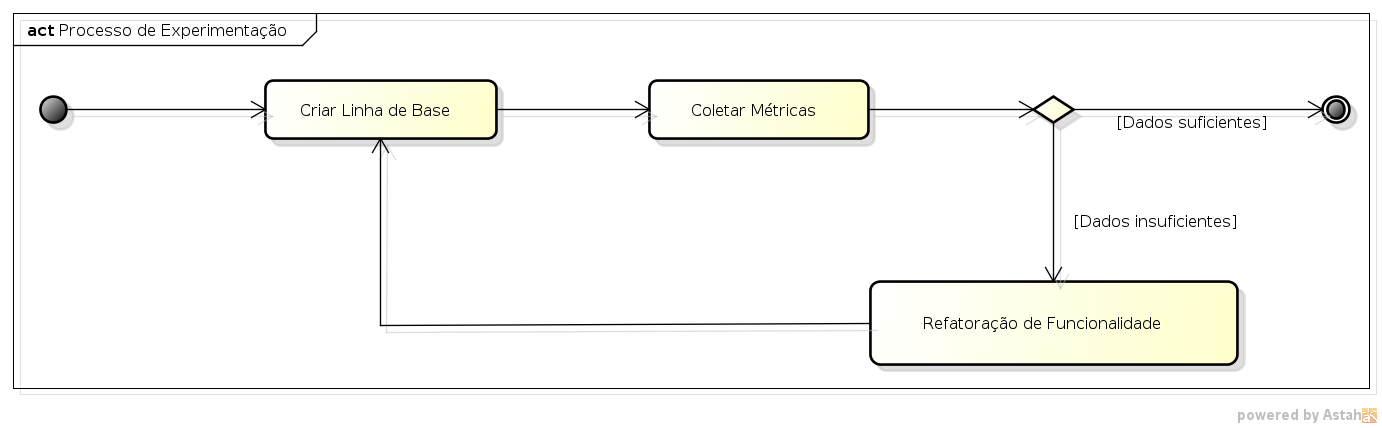
\includegraphics[scale=0.4]{img/processo_experimentacao.png}
	\caption[Processo de Experimentação]{Processo de Experimentação/Fonte: Próprio
	Autor}
	\label{processo_experimentacao}
\end{figure}

\begin{description}
\item[Definir versão de referência] - Delimitar um marco do estado do código no
repositório.
\item[Refatoração de funcionalidade] Esta atividade tem como objetivo aplicar os
padrões propostos em uma funcionalidade do aplicativo.
\item[Construir proejto] Excutar o processo de construção do projeto que inclui
a compilação das classes para fazer a coleta das métricas.
\item[Coleta de Métricas] Este passo tem como objetivo fazer a coleta
das métricas do código que se encontra no repositório a partir de uma revisão
para fazer a avaliação dos efeitos da refatoração na qualidade do código.
\item[Análise dos resultados] Discussão dos impactos das alterações executadas
nas métricas.
\end{description}


\section{Organização do Trabalho}

O presente trabalho está estruturado em 4 capítulos dos quais este é o
Capítulo 1 que apresenta a proposta do trabalho, contexto do problema, a
motivação para este estudo, os objetivos a serem alcançados e a estrutura do
trabalho. Também é abordada a metodologia aplicada neste trabalho mostrando o
objeto de estudo a ser analisado e os passos a serem executados, enfatizando o
método experimental.
O Capítulo 2 discorre sobre a fundamentação teórica sobre padrões de projetos,
métricas de qualidade orientada a objetos e as tecnologias com as quais o objeto
de estudo foi desenvolvido.
O Capítulo 3 contém uma análise do objeto de estudo e define como serão feitas
as implementações e mostra os resultados da execução da pesquisa.
O Capítulo 4 apresenta a análise final, conclusões do trabalho e sugestões para
trabalhos futuros.
